\section{Objective function and gradients of elastic WERTI}
Assume that there is a perturbation $\delta c_{ijkl}$ in the background elastic media
$c_{ijkl}$, the background wavefileds $u_i$ and perturbed wavefields
$\delta u_i$ satisfy:
\begin{equation}
    \rho \frac{\partial u^2_i}{\partial t^2}  -
    \frac{\partial}{\partial x_j}\left[ 
        c_{ijkl}\frac{\partial u_{k}}{\partial
        x_l}\right]=f_i,
    \label{eq:WE} 
\end{equation}
and
%\begin{equation}
%	\tau(\mathbf{x_r},t;\mathbf{x_s})=\frac{1}{2}\int
%	(d_{cal}(\mathbf{x_r},t;\mathbf{x_s})-d_{obs}(\mathbf{x_r},t+\tau;\mathbf{x_s}))^2dtd\mathbf{x_r}d\mathbf{x_s}
%    \label{eq:DeltaWE} 
%\end{equation}
\begin{equation}
    \rho \frac{\partial \delta u^2_i}{\partial t^2}  -
    \frac{\partial}{\partial x_j}\left[ 
        c_{ijkl}\frac{\partial \delta u_{k}}{\partial
        x_l}\right]=\frac{\partial}{\partial x_j}\left[\delta c_{ijkl}\frac{\partial u_{k}}{\partial x_l}\right],
    \label{eq:DeltaWE} 
\end{equation}
where $\delta u_i$ can be seen as the demigrated reflection data using the image
perturbation $\delta c_{ijkl}$ obtained from RTM or other image method. In WERTI, we
aim to minimize the traveltime differences between observed data
$\mathbf{d}^{o}$ and
calculated data $\mathbf{d}^{c}$, then
the objective function is:
\begin{equation}
	E=\frac{1}{2}\int\tau^2(\mathbf{x_r},t;\mathbf{x_s})dtd\mathbf{x_r}d\mathbf{x_s},
    \label{eq:Objectivefunction} 
\end{equation}
where the time differences $\tau(\mathbf{x_r},t;\mathbf{x_s})$ can be extracted
through DIW.
After a similar derivation as in \cite{Ma2013}, the gradients of equation \eqref{eq:Objectivefunction} can be expressed as:
\begin{equation}
	\frac{\partial E}{\partial c_{ijkl}}=-\int (\frac{\partial u_{i}}{\partial
	x_j}\frac{\partial \delta \psi_{k}}{\partial x_l}+\frac{\partial \delta u_{i}}{\partial
	x_j}\frac{\partial \psi_{k}}{\partial x_l}),
    \label{eq:GradientCijkl}
\end{equation}
where $\psi_i$ and $\delta \psi_i$ are the adjoint wavefields satisfying:
\begin{equation}
    \rho \frac{\partial \psi^2_i}{\partial t^2}  -
    \frac{\partial}{\partial x_j}\left[ 
        c_{ijkl}\frac{\partial \psi_{k}}{\partial
		x_l}\right]=\tau(\mathbf{x_r},t;\mathbf{x_s})\frac{\dot{d}^o_i(\mathbf{x_r},t+\tau;\mathbf{x_s})}{h_i(\mathbf{x_r},t;\mathbf{x_s})},
    \label{eq:AdjointWE} 
\end{equation}
and
\begin{equation}
    \rho \frac{\partial \delta \psi^2_i}{\partial t^2}  -
    \frac{\partial}{\partial x_j}\left[ 
        c_{ijkl}\frac{\partial \delta \psi_{k}}{\partial
        x_l}\right]=\frac{\partial}{\partial x_j}\left[\delta c_{ijkl}\frac{\partial
		\psi_{k}}{\partial x_l}\right],
    \label{eq:AdjointDeltaWE} 
\end{equation}
with
$h_i(\mathbf{x_r},t;\mathbf{x_s})=(\dot{d}^o_i(\mathbf{x_r},t+\tau;\mathbf{x_s}))^2-\ddot{d}^o_i(\mathbf{x_r},t+\tau;\mathbf{x_s})(d^c_i(\mathbf{x_r},t;\mathbf{x_s})-d^o_i(\mathbf{x_r},t+\tau;\mathbf{x_s}))$. The
hat dot denotes the time derivative. On the right hand side (RHS) of equation
\eqref{eq:GradientCijkl}, the first and second term indicate the source and receiver
part of the reflection wave-path, respectively. Then we can get the gradients in terms of P- and
S- wave velocities through the chain rule:
\begin{equation}
	\frac{\partial E}{\partial V_p}=2\rho V_p\frac{\partial E}{\partial
		c_{ijkl}}\delta_{ij}\delta_{kl}, \qquad
	\frac{\partial E}{\partial V_s}=2\rho V_s\frac{\partial
	E}{\partial c_{ijkl}}(-2\delta_{ij}\delta_{kl}+\delta_{ik}\delta_{jl}+
	\delta_{il}\delta_{jk}).
    \label{eq:GradientVel}
\end{equation}

%DIW can not provide
%reliable traveltime differences if there are too
%many intersections between different events.
\section{Workflow of elastic WERTI}
In elastic case, it is common to observe that different mode-conversions, mainly P-P
and P-S events, overlap and intersect with each other. The cross points between events
would be singularities for traveltime difference estimation through DIW.
Therefore, $\tau(\mathbf{x_r},t;\mathbf{x_s})$ would be inaccurate if using the
original multicomponent seismic data, which makes the above gradients difficult to implement.
To deal with this, we decompose the observed and calculated data into P- and S-wave
parts, respectively. The decomposition is only applied on the surface recording data
\cite[]{Li2016a}
so that we can easily get the separated vector P and S-wave seismograms for each shot.
In this way, the traveltime differences can be divided into P- and
S-wave part, with which we can implement the elastic WERTI through a two-stage
workflow, i.e. the P-wave stage followed by the S-wave stage.

In the P-wave stage, the P-P reflections are mainly used to build the P-wave velocity
model. 
Firstly, we obtain the perturbation of $V_p$ ($\delta V_p$) through 
%one-iteration EFWI. There is no need to update the $\delta V_p$ iteratively since we
%only care the traveltime but not the amplitude of the demigrated data.
elastic reverse time
migration (ERTM). Since only the traveltime is considered in WERTI, we just apply an
ERTM to obtain the image rather than a least-square ERTM to fit the amplitude of
reflections. 
Then, the objective function is changed to minimize the P-P reflection traveltime differences:
\begin{equation}
	E_{pp}=\frac{1}{2}\int\tau^2_{pp}(\mathbf{x_r},t;\mathbf{x_s})dtd\mathbf{x_r}d\mathbf{x_s}.
    \label{eq:ObjectivefunctionPP} 
\end{equation}
Thus, we can obtain the gradient of  $V_p$, $\frac{\partial E}{\partial
V_p}$, just using the P-wave seismograms to
calculate RHS of equation \eqref{eq:AdjointWE} and replacing $\delta c_{ijkl}$ with
$\delta V_p$ in equation \eqref{eq:DeltaWE} and \eqref{eq:AdjointDeltaWE}.

In the S-wave stage, a similar strategy is applied using the P-S reflection
traveltime. The objective function becomes:
\begin{equation}
	E_{ps}=\frac{1}{2}\int\tau^2_{ps}(\mathbf{x_r},t;\mathbf{x_s})dtd\mathbf{x_r}d\mathbf{x_s}.
    \label{eq:ObjectivefunctionPS} 
\end{equation}
However, the implementation is a little different from the previous stage. After the
P-wave stage inversion, the background $V_p$ should be well recovered. As we know, in
most cases $V_p$ and $V_s$ share a same structure in the subsurface. Therefore, we
recommend to use the well imaged $\delta V_p$ instead of $\delta V_s$ to generate the P-S reflections. 
Besides, in the P-S reflection, the source part of the wavepath only relates to P-wave velocity so
that we can drop the first term in the RHS of equation \eqref{eq:GradientCijkl} when
calculating $\frac{\partial E}{\partial V_s}$. And also wave mode decomposition is
applied to make sure that only S-wave energy are involved:
\begin{equation}
	\frac{\partial E_{ps}}{\partial V_s}=-2\rho V_s
	\int (\frac{\partial \delta u^S_{i}}{\partial
    x_j}\frac{\partial \psi^S_{k}}{\partial x_l})
	(\delta_{ik}\delta_{jl}+
	\delta_{il}\delta_{jk}).
    \label{eq:GradientVel}
\end{equation}
The above gradient is similar to the EFWI proposed by \cite{Wang2015a}. The mode
decomposition can mitigate parameter trade-offs and suppress artifacts for the
$V_s$ inversion.
\begin{figure}
   \centering
   \subfigure[]{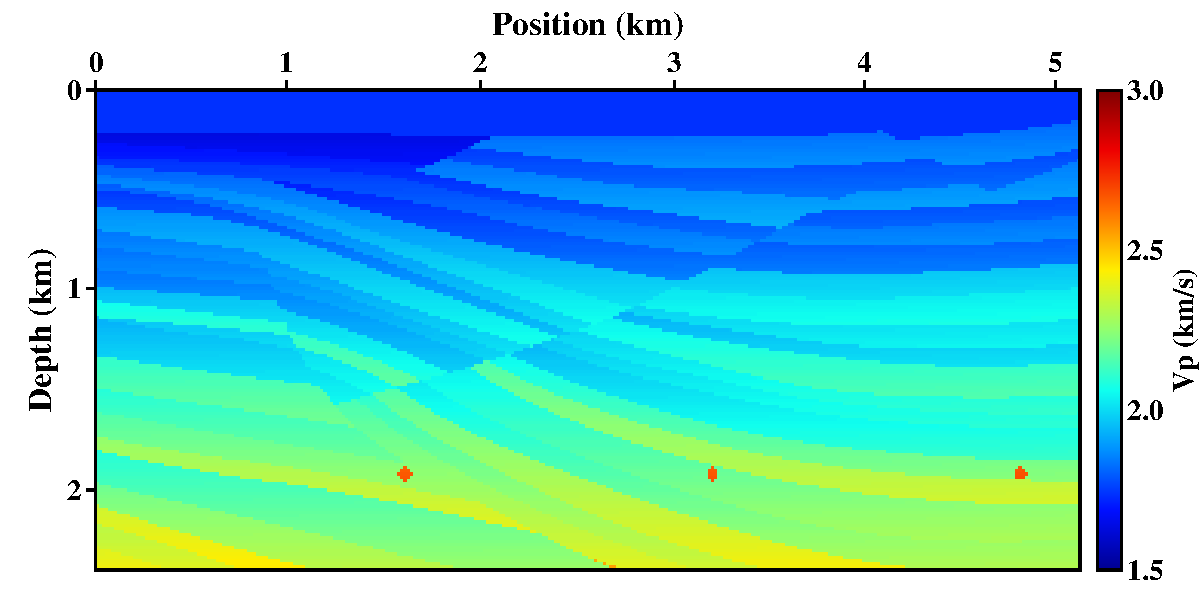
\includegraphics[width=0.48\textwidth]{sigbee2/Fig/cuttruevp.pdf}}
   \subfigure[]{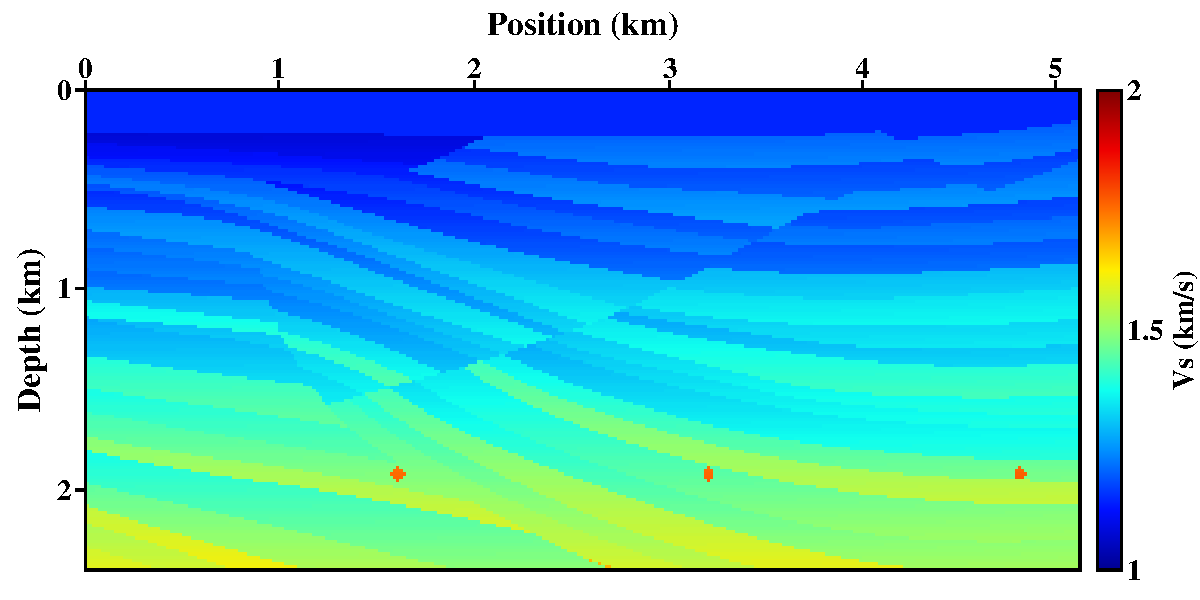
\includegraphics[width=0.48\textwidth]{sigbee2/Fig/cuttruevs.pdf}}
   \subfigure[]{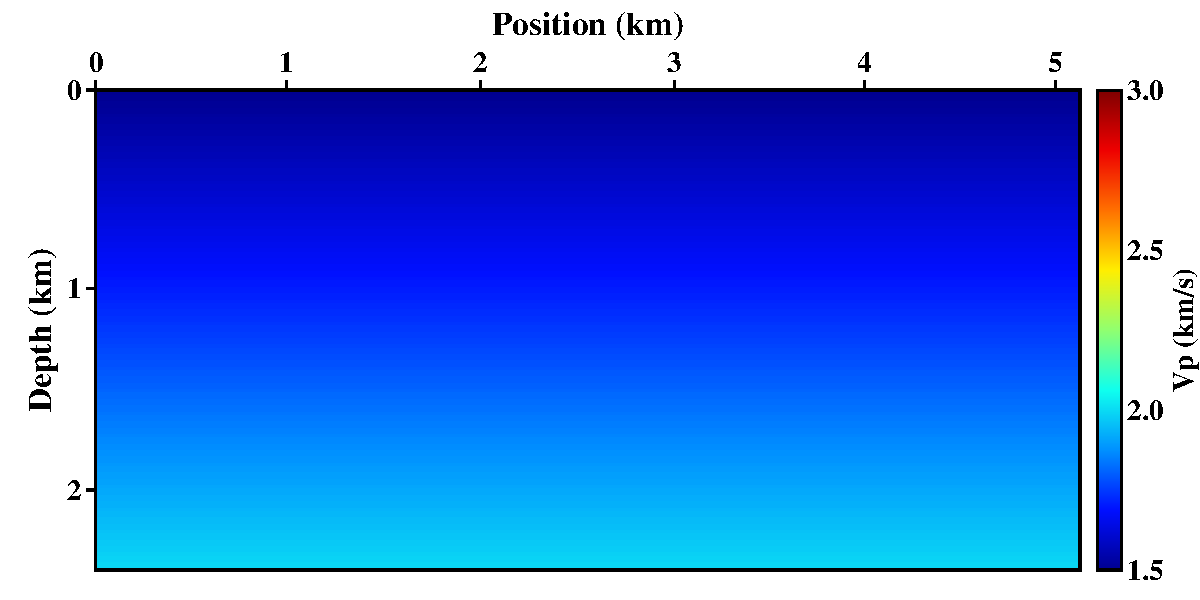
\includegraphics[width=0.48\textwidth]{sigbee2/Fig/cutinitvp.pdf}}
   \subfigure[]{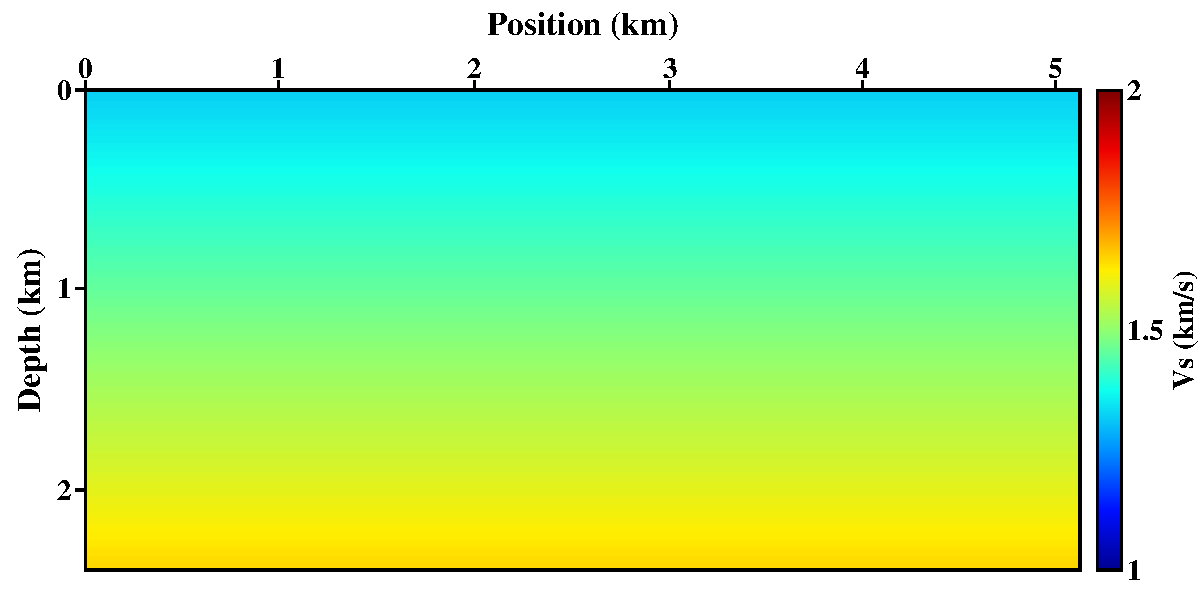
\includegraphics[width=0.48\textwidth]{sigbee2/Fig/cutinitvs.pdf}}
   \caption{Sigbee2A model example. On the top are true models of 
   $V_p$ (a) and $V_s$ (b). On the bottom are initial models of $V_p$ (c) and $V_s$
   (d) linearly increasing with depth. }
   \label{fig:TrueAndInitial}
\end{figure}

\section{Sigbee2A model example}
The synthetic example involves a part of the Sigsbee2A model (Figure
\ref{fig:TrueAndInitial}a and \ref{fig:TrueAndInitial}b).
The $V_s$ model is generated using fixed Poisson's ratio. Figure
\ref{fig:TrueAndInitial}c and \ref{fig:TrueAndInitial}d show the initial model of
$V_p$ and $V_s$, which linearly increase with depth. We can see the initial
model of $V_p$ is lower while the initial model of $V_s$ is higher than the true model, but both of
them is far from the true value. 36 shots are evenly deployed on the surface with
a maximum offset of 4km. Pure P-wave source is used with a main frequency of 15Hz.

Figure \ref{fig:InvertedModel}a and \ref{fig:InvertedModel}b show the inverted results of elastic WERTI.
Since the linearly increased initial model is quite far from the true value, certainly there will be
cycle-skipping problem if we use this for conventional EFWI. However, after
40 iteration for each stage, WERTI provides a good recovery of the background
information for both $V_p$ and $V_s$. Using the inverted results of WERTI as starting
models, we also perform the conventional EFWI. As shown in Figure \ref{fig:InvertedModel}c and
\ref{fig:InvertedModel}d, both of the inverted $V_p$ and $V_s$ models are well
reconstructed except the right part.
The reason should be that, on the right part, the reflection coverage of surface observation is insufficient for
WERTI to rebuild the long-wavelength components. 
Figure \ref{fig:Profiles} shows the vertical profiles at 1.5km and 3km. 
We can see that the elastic WERTI provides reliable starting models containing long-wavelength
components for EFWI and the EFWI results match well with the true value.
\begin{figure}[!htb]
   \centering
   \subfigure[]{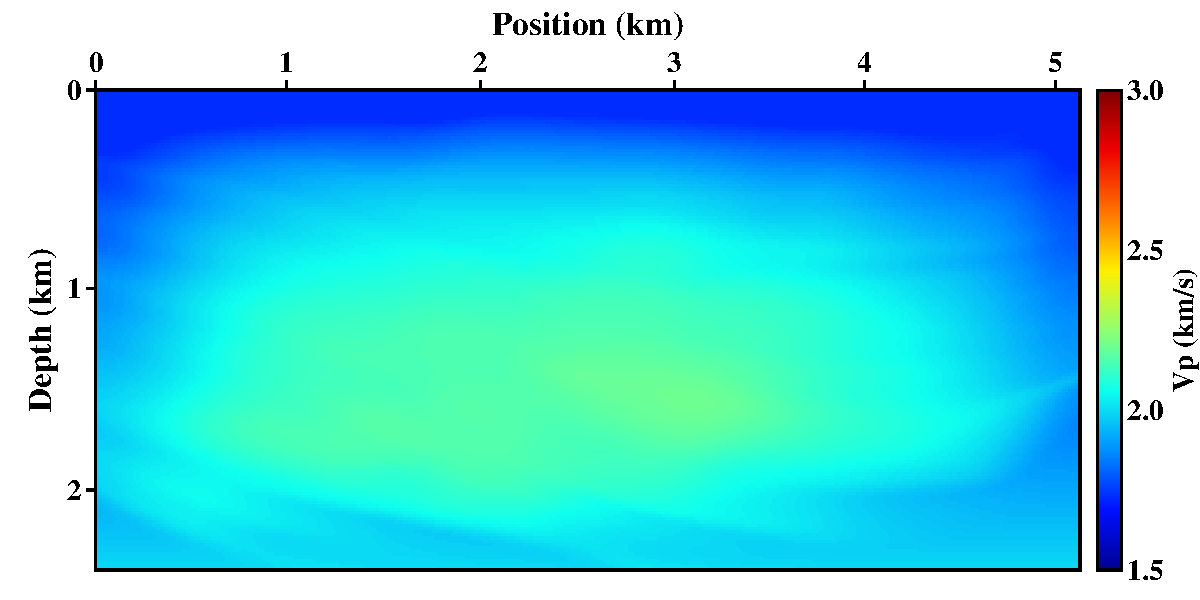
\includegraphics[width=0.48\textwidth]{sigbee2/Fig/newinit3vp.pdf}}
   \subfigure[]{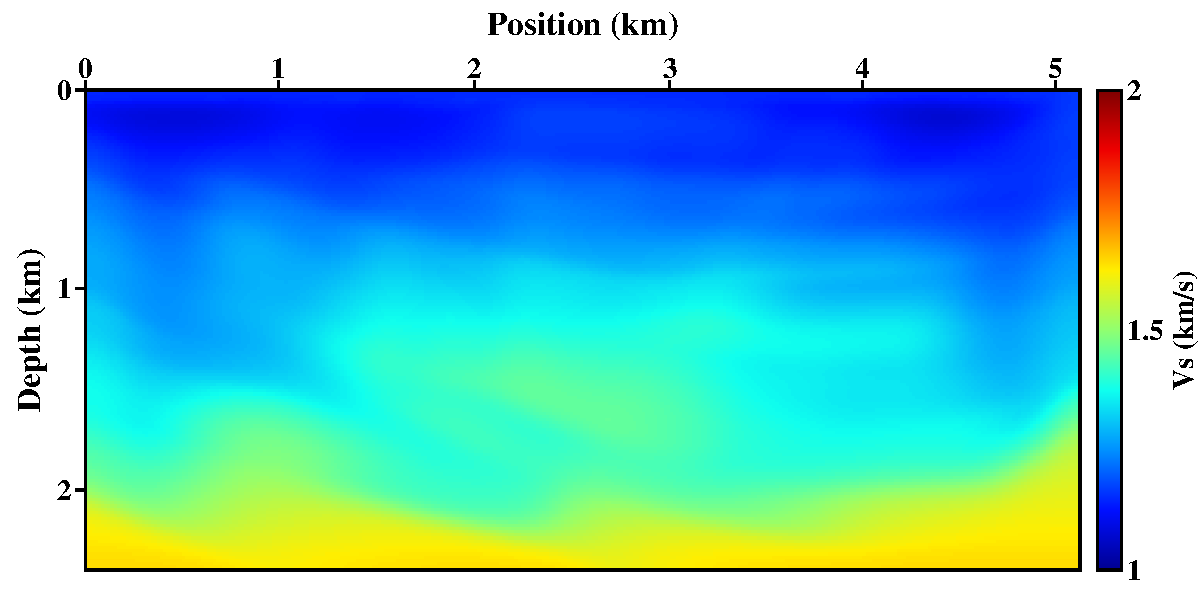
\includegraphics[width=0.48\textwidth]{sigbee2/Fig/newinit3vs.pdf}}
   \subfigure[]{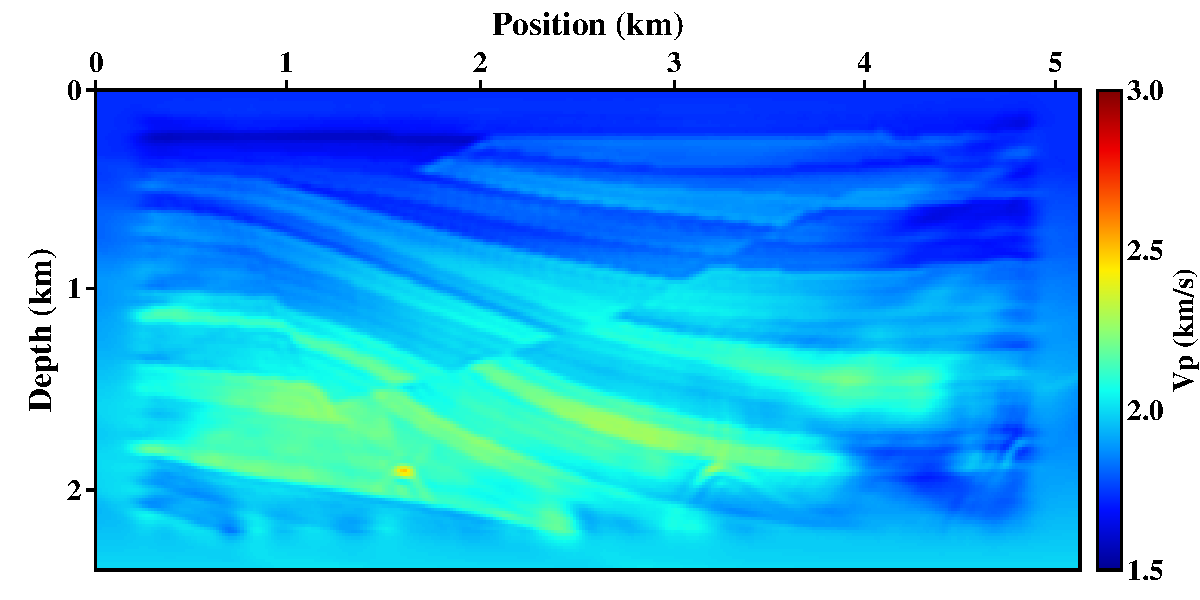
\includegraphics[width=0.48\textwidth]{sigbee2/Fig/nodevp.pdf}}
   \subfigure[]{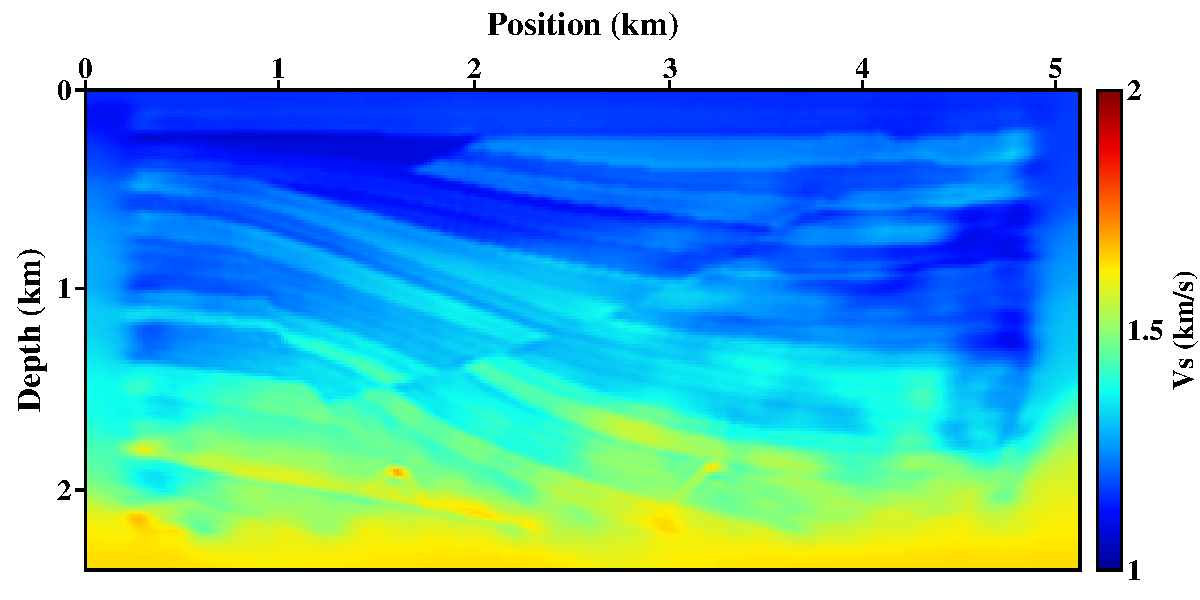
\includegraphics[width=0.48\textwidth]{sigbee2/Fig/nodevs.pdf}}
   \caption{Inverted results of WERTI and EFWI. (a) and (b) are inverted $V_p$ and
	   $V_s$ model through two-stage elastic WERTI with the linearly increased models
	   as initial models. (c) and (d) are inverted $V_p$ and $V_s$ through EFWI using
   (a) and (b) as starting models.}
   \label{fig:InvertedModel}
\end{figure}
\begin{figure}[!htb]
   \centering
   \subfigure[]{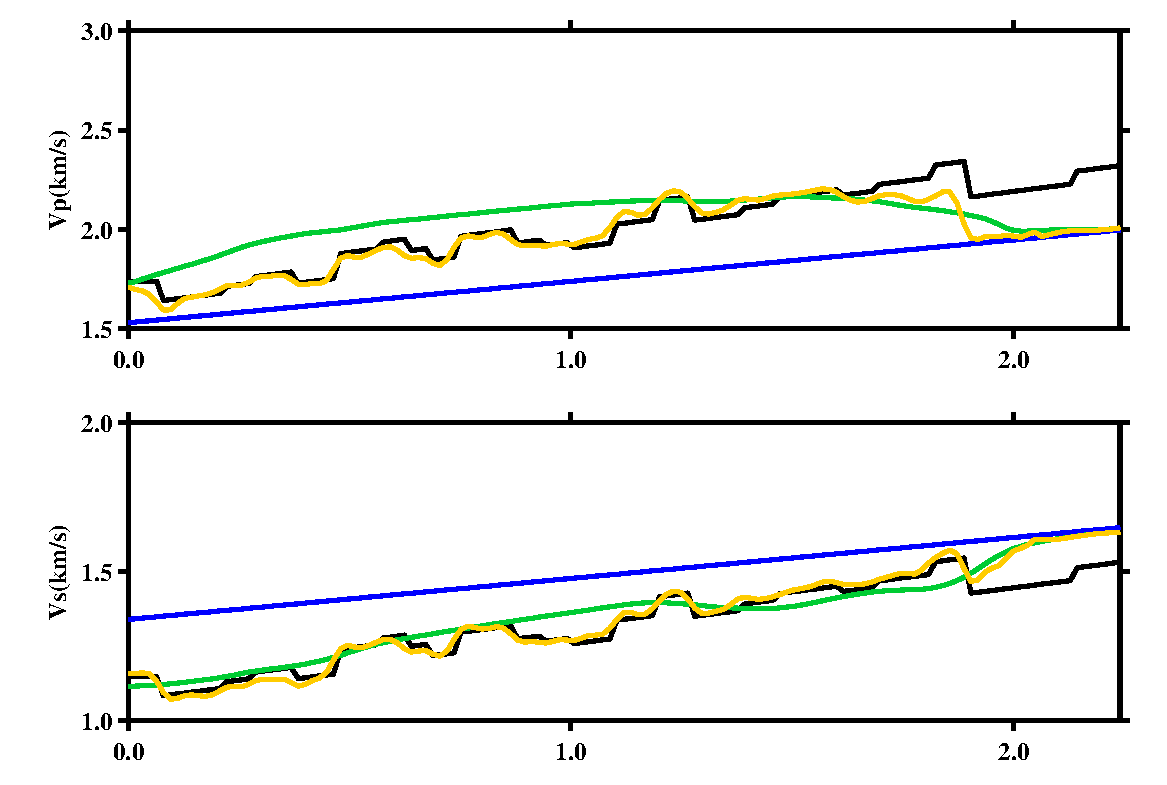
\includegraphics[width=0.48\textwidth]{sigbee2/Fig/1km.pdf}}
   \subfigure[]{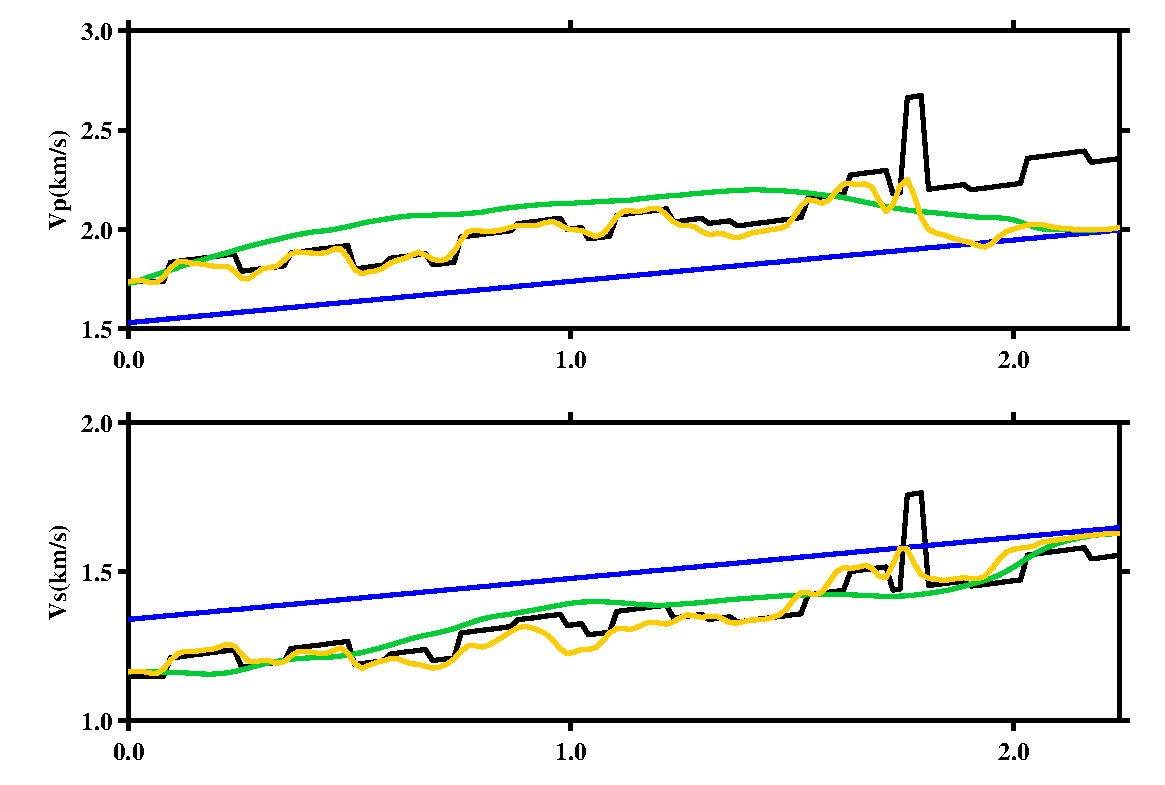
\includegraphics[width=0.48\textwidth]{sigbee2/Fig/3km.pdf}}
   \caption{Vertical profiles of elastic WERTI and EFWI results at 1.4km (a) and
	   3km (b). The black and blue lines indicate the true and linearly increased
	   initial model. The green and yellow lines indicate the WERTI and EFWI results,
	   respectively.
   }
   \label{fig:Profiles}
\end{figure}
\section{Conclusions}
Reflection traveltime inversion only minimizes traveltime misfits which are more sensitive
and linearly related to the low-wavenumber model perturbation. With the aid of DIW and
P/S separation of 3C seismograms, we can obtain the travel time differences of P-P and P-S
reflections, respectively. 
To build the long-wavelength component of the model, we introduce a two-stage WERTI
workflow by firstly using P-P then P-S reflections. In the second stage, the wave mode
decomposition can mitigate parameter trade-offs and suppress artifacts when
calculating gradient of $V_s$.
The Sigsbee2A model example proves that even starting with a bad initial model, the
two-stage elastic WERTI strategy can provide reliable starting model for conventional EFWI. 

\section{Acknowledgement}
This work is supported by the
National Natural Science Foundation of China (NO.41474099, 41674117 \& 41630964). 
This paper is also based upon the work supported by the King Abdullah University of Science
and Technology (KAUST) Office of Sponsored Research (OSR) under award NO. 2230.
We appreciate the open-source package of DENISE from
\textit{https://github.com/daniel-koehn/} and Mines Java Toolkit from
\textit{https://github.com/dhale}.
We thank the useful advice from Tariq Alkhalifah (KAUST), Zedong Wu (KAUST) and Benxin Chi (Los Alamos).


